% !TEX root = ../thesis.tex
%
\chapter{Application}
\label{sec:application}
\begin{figure}[h!]
    \centering
    \begin{tabulary}{\textwidth}{cc}
        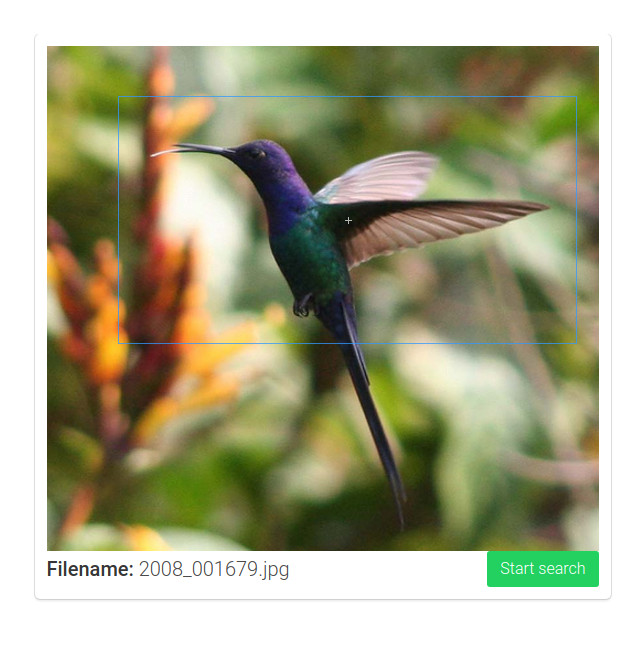
\includegraphics[height=4.5cm]{figures/server_select} &
        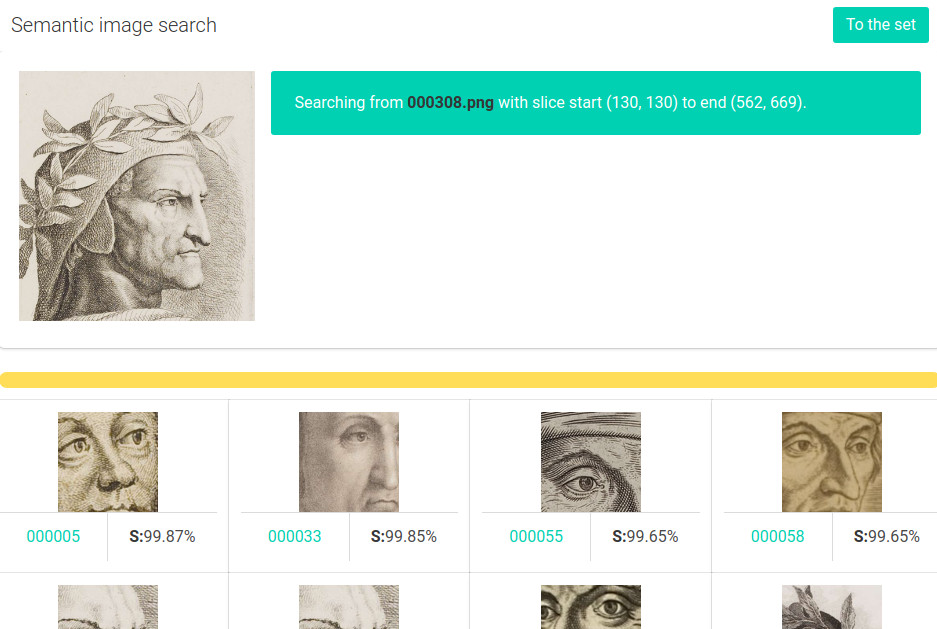
\includegraphics[height=4.5cm]{figures/server_results}
    \end{tabulary}
    \caption{Two screenshots of the provided online app using our method. Left shows the selection screen previous to a new search. Right shows the result screen displaying live results.}
    \label{fig:application}
\end{figure}
We bring the described method to application as a semantic image search machine. For this we build a small exemplar web application using the Flask microframework.\\
After configuring the program for a new image database, the web application enables users to search for similar objects given a query image patch. In the main view the user can sift through the image dataset to pick an image which contains the object of interest. For a single image the \gls{gui}\fref{fig:application} provides a intuitive way to select a rectangular part of an image. Alternatively the user may upload an image to the web page, to search the database with an external image. Next the user can start the search with the provided patch. The backend quickly fine-tunes the \gls{resnet} under the same conditions as described in \treft{sec:results}. Because we do not have any semantic information about the images or the objects seen in them we can not yield guaranteed negative samples given a query patch. Thereby we resort to random patches that we randomly sample at different sizes from the whole dataset. In training we pick 500 seed patches from the query image so that we can set those against a equal number of random chosen negatives. We assume that even with some actual positive under the negatives, the high number of samples lowers their influence in training.\\
Following the training, the network is instantly reshaped into the \gls{fcn} and set up for normal image forwarding. The images from the database are all forwarded through the detection pipeline. While the network is still running the program collects the best results and presents the patches with the highest score to the user, in descending order by their scores.

\section{Retrieval examples}
\label{sec:application:examples}
\begin{figure}[htb]
    \setlength\tabcolsep{3pt}
    \renewcommand{\arraystretch}{0}
    \begin{tabular}{c|ccccc}
      \appim{portraits/000308_165_232_552_637} &
      \appim{portraits/000005_200_450_300_550_pick} &
      \appim{portraits/000036_300_500_400_600_pick} &
      \appim{portraits/000055_250_450_350_550_pick} &
      \appim{portraits/000053_400_350_500_450_pick} &
      \appim{portraits/000033_300_396_400_529_pick} \\

      \appim{sspiegel/000446_218_115_389_257} &
      \appim{sspiegel/000011_800_150_900_250_blurred} &
      \appim{sspiegel/000538_850_200_950_300_blurred} &
      \appim{sspiegel/000479_100_100_200_200_blurred} &
      \appim{sspiegel/000465_550_200_650_300_blurred} &
      \appim{sspiegel/000465_400_100_500_200_blurred} \\

      \appim{voc/2008_003088_16_37_332_412} &
      \appim{voc/2010_001794_150_250_250_350_blurred} &
      \appim{voc/2008_000724_100_264_200_397_blurred} &
      \appim{voc/2009_001444_150_150_250_250_blurred} &
      \appim{voc/2009_004639_200_250_300_350_blurred} &
      \appim{voc/2009_003419_150_150_250_250_blurred} \\
    \end{tabular}
	\caption{The first patch on the left is the query image. Right are the five highest scoring retrievals cutted to show the context. The actual proposed patches are drawn sharp on the blurred source images.}
  \label{fig:retrieval}
\end{figure}
Returning to the objective domain of this thesis we set up our application with two dataset of art historical images. The first is a collection of drawn or printed portrait illustrations containing 923 images. The second consists of 567 scans of pages from the \textit{Sachsenspiegel}     \citep{von_repgow_heidelberger_????}, a German law book from the 13th century.\\
\figreft{fig:retrieval} displays some qualitative examples from those sets. With the retrieved patches the presence of too small bounding boxes \tref{sec:results:results} again becomes apparent. Observe in the first row how from the query portrait of \textit{Dante}, three other portraits of \textit{Dante} were retrieved (the second retrieval is from a different image depicting the same portrait). The second row shows a failed example from the \textit{Sachsenspiegel} set. Generally most tests with this dataset proved to be unsuccessfully. Without further investigation we suspect that might derive from the overall similarity of the depicted figures and the fact that most images are substantially filled with text which therefore  make up considerable number of the negative training samples.

At last we show an example of a cat from the \textsc{Pascal}-VOC dataset which exclusivity retrieves cats for the at least top-hundred matches.
